\subsection{a)}

\begin{equation}
\label{eq:partSt}
\frac{\partial S}{\partial t} = b(S+I)-cS -\frac{S(I+S)}{K}-aSI + D\nabla^2S,
\end{equation}

\begin{equation}
\label{eq:partIt}
\frac{\partial I}{\partial t}= -cI -\frac{I(I+S)}{K}+aSI +D\nabla^2I.
\end{equation}

For the spatially homogeneous model, that is $D=0$ we have the steady states when

$$
\frac{\partial S^*}{\partial t}=b(S^*+I^*)-cS^*-\frac{S^*(I^*+S^*)}{K}-aS^*I^* =0
$$

and

$$
\frac{\partial I^*}{\partial t}=-cI^*-\frac{I^*(I^*+S^*)}{K}+aS^*I^*=0.
$$

We can directly rule our the steady states which involve $S^*=0$ or $S^*<0 \vee I^*<0$.

\begin{itemize}
\item $S^*_1=K(c-b), \;\; I^*_1=0$
\item $S^*_2=\frac{b}{a}, \;\; I^*_2=K(b-c)-\frac{b}{a}$ 
\end{itemize}



TO see the stability of these steady states we need to consider the jacobian for thses states,

\begin{equation}
\mathbb{J}^*_n=\left.\left(
\begin{array}{cc}
\frac{\partial f}{\partial S} & \frac{\partial f}{\partial I} \\
\frac{\partial g}{\partial S} & \frac{\partial g}{\partial I}
\end{array}\right)\right|_{(S^*_n,I^*_n)},
\end{equation}

where 

\begin{equation}
f(S,I)=b(S+I)-cS-\frac{S(I+S)}{K}-aSI
\end{equation}

\begin{equation}
g(S,I)=-cI-\frac{I(I+S)}{K}+aSI.
\end{equation}

So
\begin{equation}
\mathbb{J}^*_n=\left.\left(
\begin{array}{cc}
b-c-\frac{I+2S}{K}-aI & b-\frac{S}{K}-aS \\
-\frac{I}{K} +aI & -c -\frac{2I+S}{K}+aS
\end{array}\right)\right|_{(S^*_n,I^*_n)},
\end{equation}

To have a stable steady state we need that 

\begin{enumerate}
\item $Tr(\mathbb{J}^*_n)<0$
\item $Det(\mathbb{J}^*_n)>0$
\end{enumerate}


For $n=1$ we get that the steady state is stable for

$$
K>\frac{3c}{a(c-b)}
$$$$
K<\frac{2c-b}{a(c-b)}
$$

which can't be fulfilled at the some time.


\begin{equation}
K_c=Max\left[\frac{b}{a(b-c)},\frac{2b-3c}{a(b-c)}\right]
\end{equation}

From steady state $n=2$.
\subsection{b)}

Change of variables $N=I+S$ inserted into equations \eqref{eq:partIt} and \eqref{eq:partSt} gives,

\begin{equation}
\frac{\partial N}{\partial t}=bN -cN -\frac{N^2}{K}+D\nabla^2N.
\end{equation}

If we assume that we are studying the dynamics in one dimension, we can replace the $\nabla^2$ operator with a second derivative in that direction, i.e. $\nabla^2\rightarrow \frac{\partial^2}{\partial x^2}$ and we get the time evolution as,

\begin{equation}
\frac{\partial N}{\partial t}=(b-c)N\left(1-\frac{N}{K}\right)+D\frac{\partial^2 N}{\partial x^2}.
\end{equation}

To see if the dynamics exhibits a travelling wave solution we try to reduce the spatial and temporal dimension to one by $z=x-ct$ which would yield,

\begin{equation}
-c\frac{\partial N}{\partial z}=(b-c)N\left(1-\frac{N}{K}\right)+D\frac{\partial^2 N}{\partial x^2}.
\end{equation}

To study the dynamics of this system we write it with a new variable $v=\frac{\partial n}{\partial z}$ and receive the system 

\begin{align*}
\frac{\partial n}{\partial z}&=v\\
\frac{\partial v}{\partial z}&=-\frac{c}{D}v-\frac{(b-c)n(1-\frac{n}{K})}{D}.
\end{align*}

This system has the steady states 

\begin{equation}
c_s>\sqrt{4D(b-c)} \Rightarrow c_s>\sqrt{2}
\end{equation}

\subsection{c)}
%
%\begin{figure}[h]
%    \centering
%    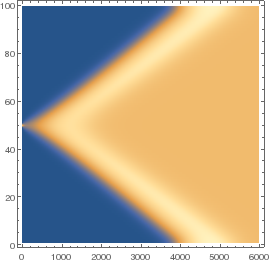
\includegraphics[width=0.45\textwidth]{img/listdensityplot_S.eps}
%    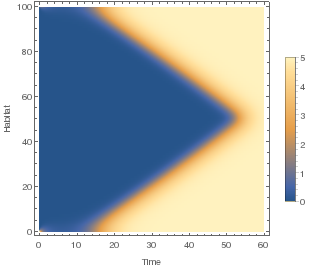
\includegraphics[width=0.45\textwidth]{img/listdensityplot_P.eps}
%  \caption{}
%\end{figure}

\begin{figure}
\centering
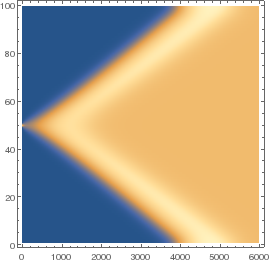
\includegraphics[scale=0.5]{img/listdensityplot_S.png}
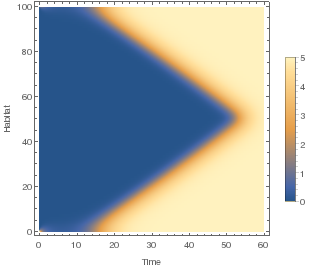
\includegraphics[scale=0.5]{img/listdensityplot_P.png}
\caption{\label{fig:pic1c}}
\end{figure}